\chapter{Rendszertesztek és bemutató szcenáriók}

\section{Tesztek megvalósítása}
A cél annak igazolása, hogy a rendszer komponensei megfelelően működnek. 
A vizsgálat során \emph{idősoros} bemeneti (\texttt{esp\{x\}\_schedule.txt}) és kimeneti 
fájlt (\texttt{thresholds.txt}) használunk. 
Ebben az esetben a kontrollciklus periódusa \(T_c=3\,\mathrm{s}\).

Mérőszámok és ellenőrzési pontok:
\begin{itemize}
  \item \textbf{Összáram} (\texttt{sum\_current\_amps}) és \textbf{mérőnkénti tényleges áram} (\texttt{effective}) 
  a vezérlő \texttt{/status} végpontján és az \texttt{output.txt}-ben.
  \item \textbf{Korlátok (cap)}: az allokáció (max--min fair) eredményei.
  \item \textbf{Küszöbök}: \texttt{ALLOC\_MAX\_TOTAL}, \texttt{BREAKER\_MAX\_TOTAL}, \texttt{BREAKER\_MIN\_TOTAL}.
  \item \textbf{Megszakító állapot}: \texttt{on/off} (hiszterézis).
\end{itemize}

Ezeket \texttt{output.txt} idősoros naplóban ellenőriztem, itt volt a legegyszerűbb, 
mert itt egy sor egy ciklus.

\section{Bemenetek és állapot}
\begin{itemize}
  \item \texttt{thresholds.txt}: \texttt{BREAKER\_MAX\_TOTAL}, 
  \texttt{BREAKER\_MIN\_TOTAL}, \texttt{ALLOC\_MAX\_TOTAL}.
  \item \texttt{esp1\_schedule.txt}, \texttt{esp2\_schedule.txt}, \
  texttt{esp3\_schedule.txt}: \texttt{idő\ \ \ áramerősség} párok.
  \item \texttt{sim\_control.txt}: \texttt{RUNNING}/\texttt{STOPPED}; alapértelmezés: \texttt{STOPPED}.
\end{itemize}

\section{Várt viselkedés (rövid)}
\begin{enumerate}
  \item Ha \(\sum d_i \le \texttt{ALLOC\_MAX\_TOTAL}\)\,: \emph{nincs korlát} 
  (cap \(\to\) nagy érték), \(\mathrm{effective}_i=d_i\).
  \item Ha \(\sum d_i > \texttt{ALLOC\_MAX\_TOTAL}\)\,: \emph{max--min fair} 
  (water-filling) elosztás: \(a_i=\min\{d_i,\lambda\}\), \(\sum_i a_i = \texttt{ALLOC\_MAX\_TOTAL}\).
  \item Megszakító: ha \(\mathrm{sum} \ge \texttt{BREAKER\_MAX\_TOTAL}\)\,→ \texttt{off}, 
  ha \(\mathrm{sum} \le \texttt{BREAKER\_MIN\_TOTAL}\)\,→ \texttt{on}.
  \item \texttt{STOPPED} állapotban a  virtuális idő nem halad, 
  a vezérlő nem küld új cap-et és nem kapcsolgat megszakítót.
\end{enumerate}

\section{Szcenáriók és elfogadási kritériumok}

\subsection{Alaptesztek: Start/Stop/Reset/Clear}
\textbf{Bemenetek:}\\ \texttt{BREAKER\_MAX\_TOTAL=12}, \texttt{BREAKER\_MIN\_TOTAL=2}, 
\texttt{ALLOC\_MAX\_TOTAL=30}; ESP1=1.0 A, ESP2=1.5 A, ESP3=0.5 A.\\
\textbf{Lépések:}\\ STOP \(\to\) Reset \(t{=}0\) \(\to\) START.\\
\textbf{Várt eredmény:}\\ nincs korlát (cap \(\approx\) INF), Sum \(\approx 3.0\) A, 
megszakítók \texttt{on}.\\
\textbf{Siker:}\\ élő grafikonon vízszintes \(\approx 3\) A; \texttt{/status} tükrözi, 
az \texttt{output.txt} 3 s-enként bővül.

\begin{figure}[H]
    \centering
    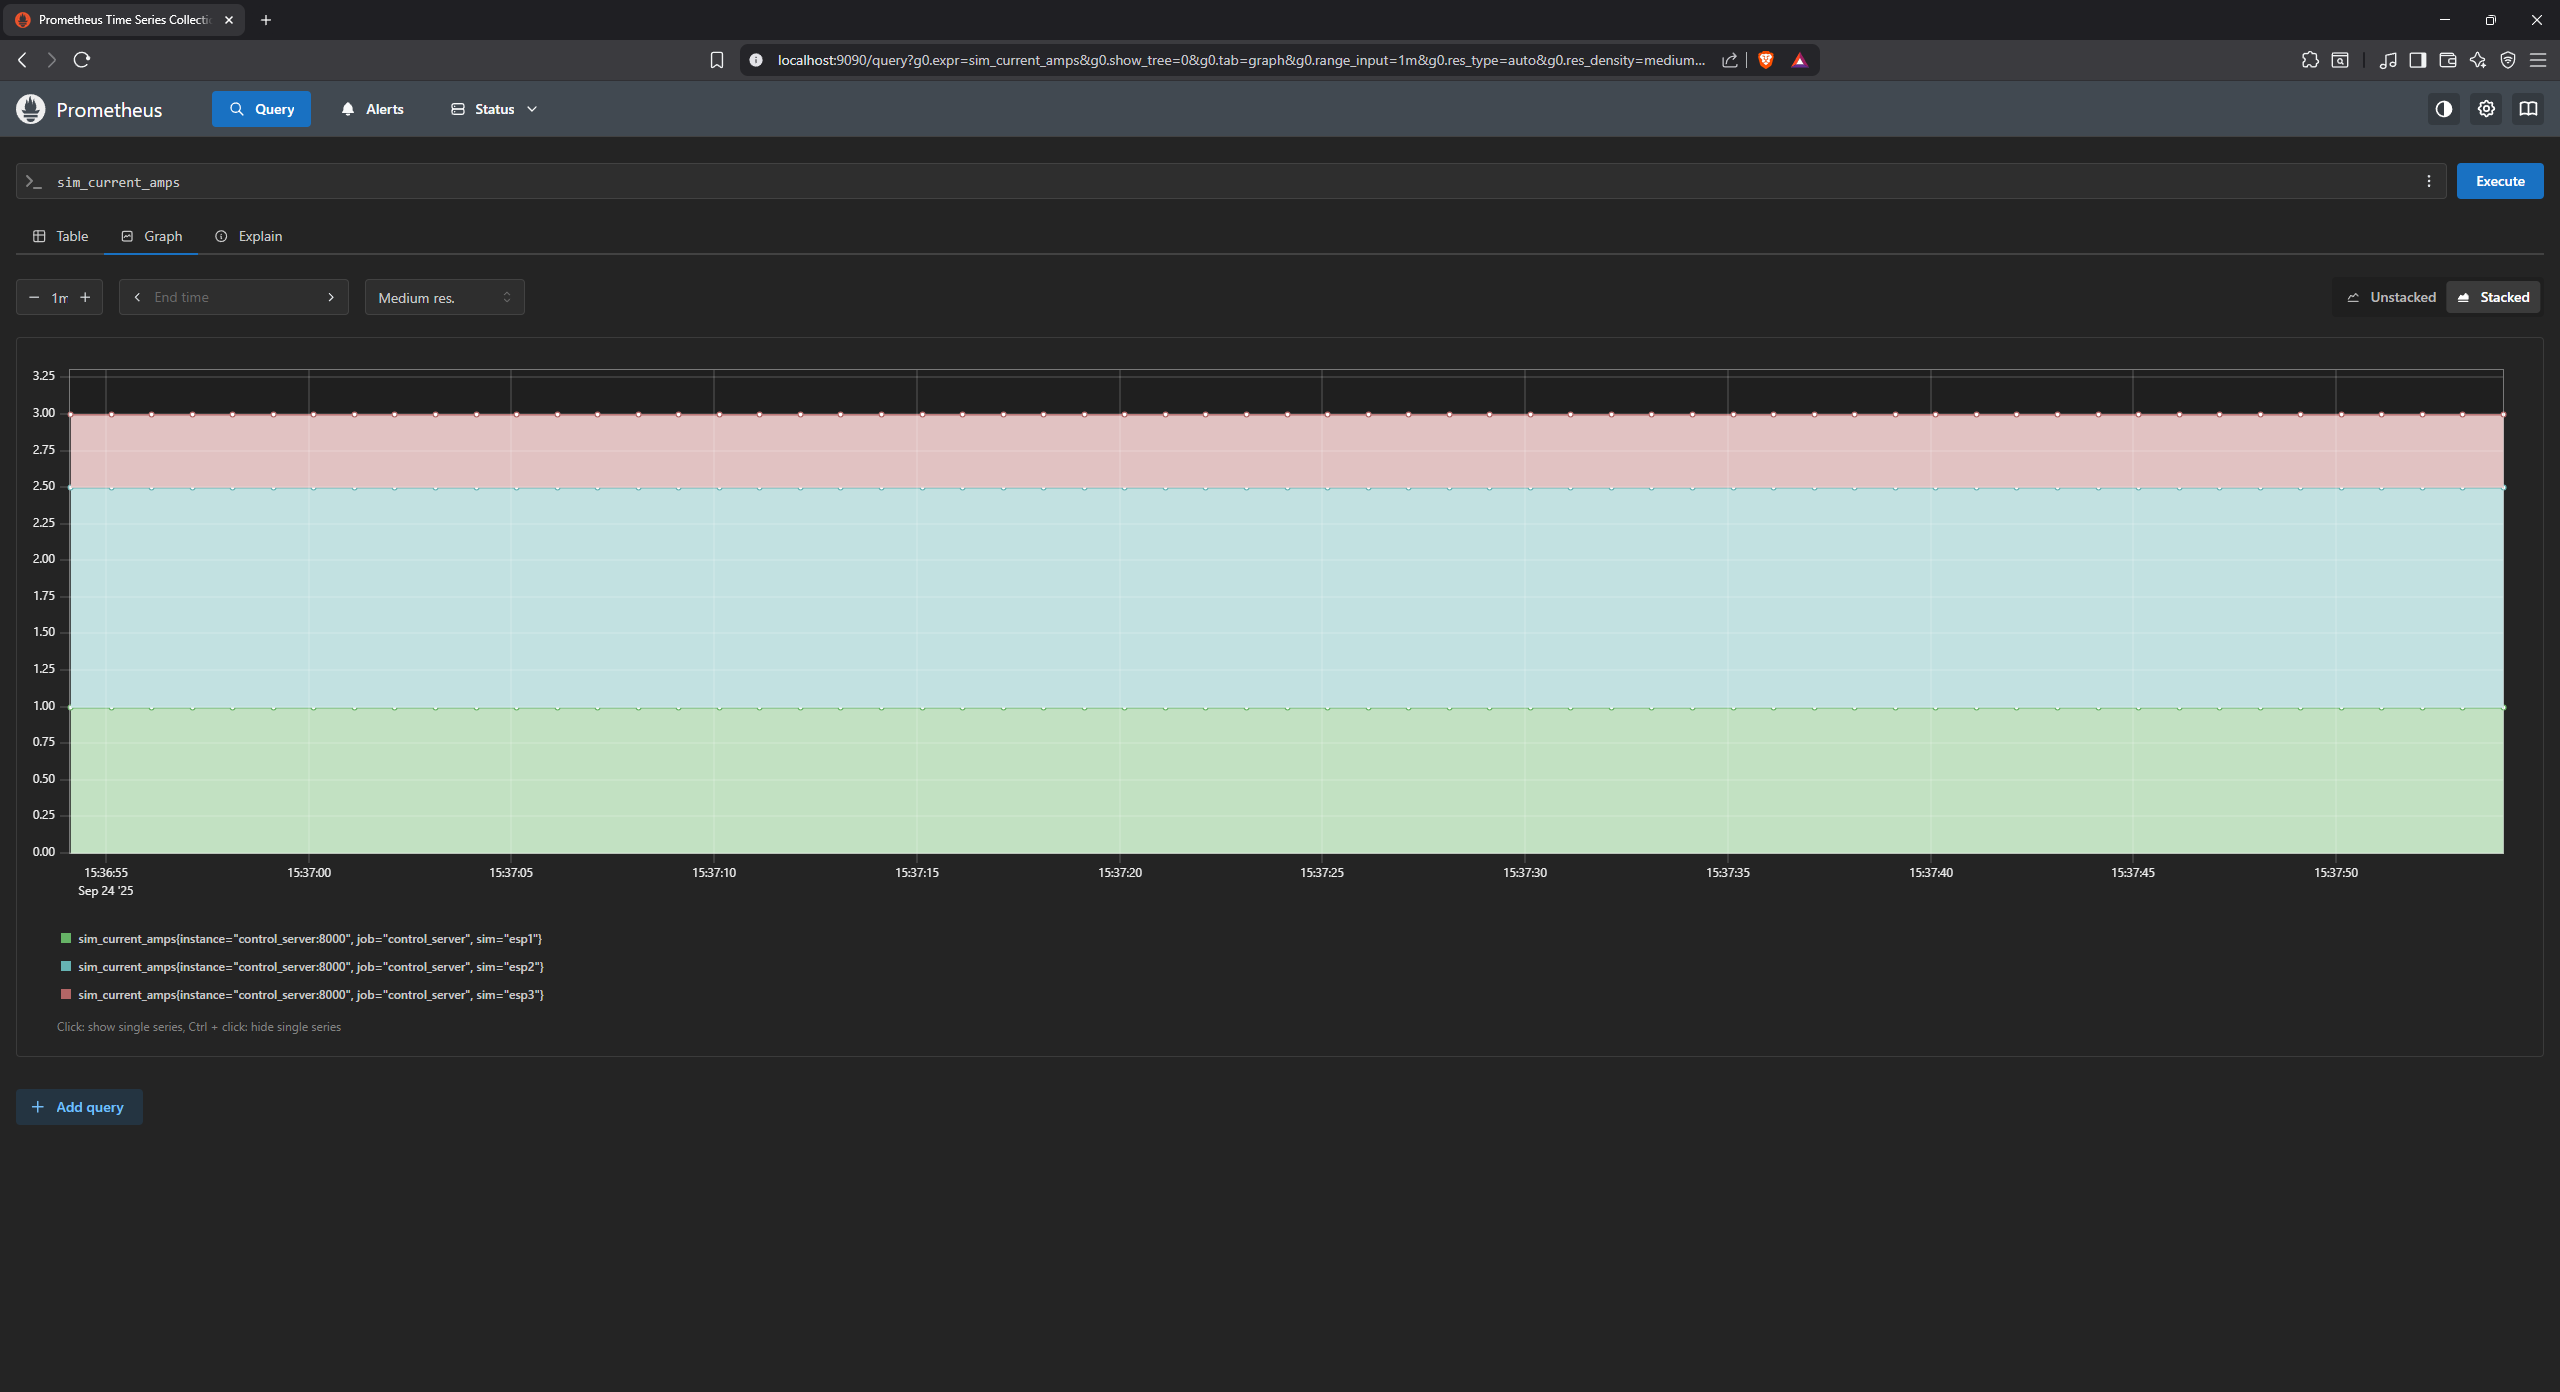
\includegraphics[width=1\textwidth]{figures/alaptesztek_1.png}
    \caption{Alaptesztek}
    \label{fig:alaptesztek}
\end{figure}

\subsection{Alulterhelés: nincs korlátozás}
\textbf{Bemenetek:}\\ \texttt{ALLOC\_MAX\_TOTAL=6}, \texttt{BREAKER\_MAX\_TOTAL=12}, 
\texttt{BREAKER\_MIN\_TOTAL=2}; ESP1=2.0 A, ESP2=1.5 A, ESP3=0.5 A (Sum=4.0 A).\\
\textbf{Lépések:}\\ START, várakozás \(\sim\) 2 ciklus.\\
\textbf{Várt eredmény:}\\ \(\mathrm{effective}_i = d_i\), cap \(\approx\) INF.\\
\textbf{Siker:}\\ \texttt{output.txt}-ben minden szimulátornál \texttt{cap} nagy (``nincs korlát''); 
grafikonon Sum \(\approx 4\) A.

\begin{figure}[H]
    \centering
    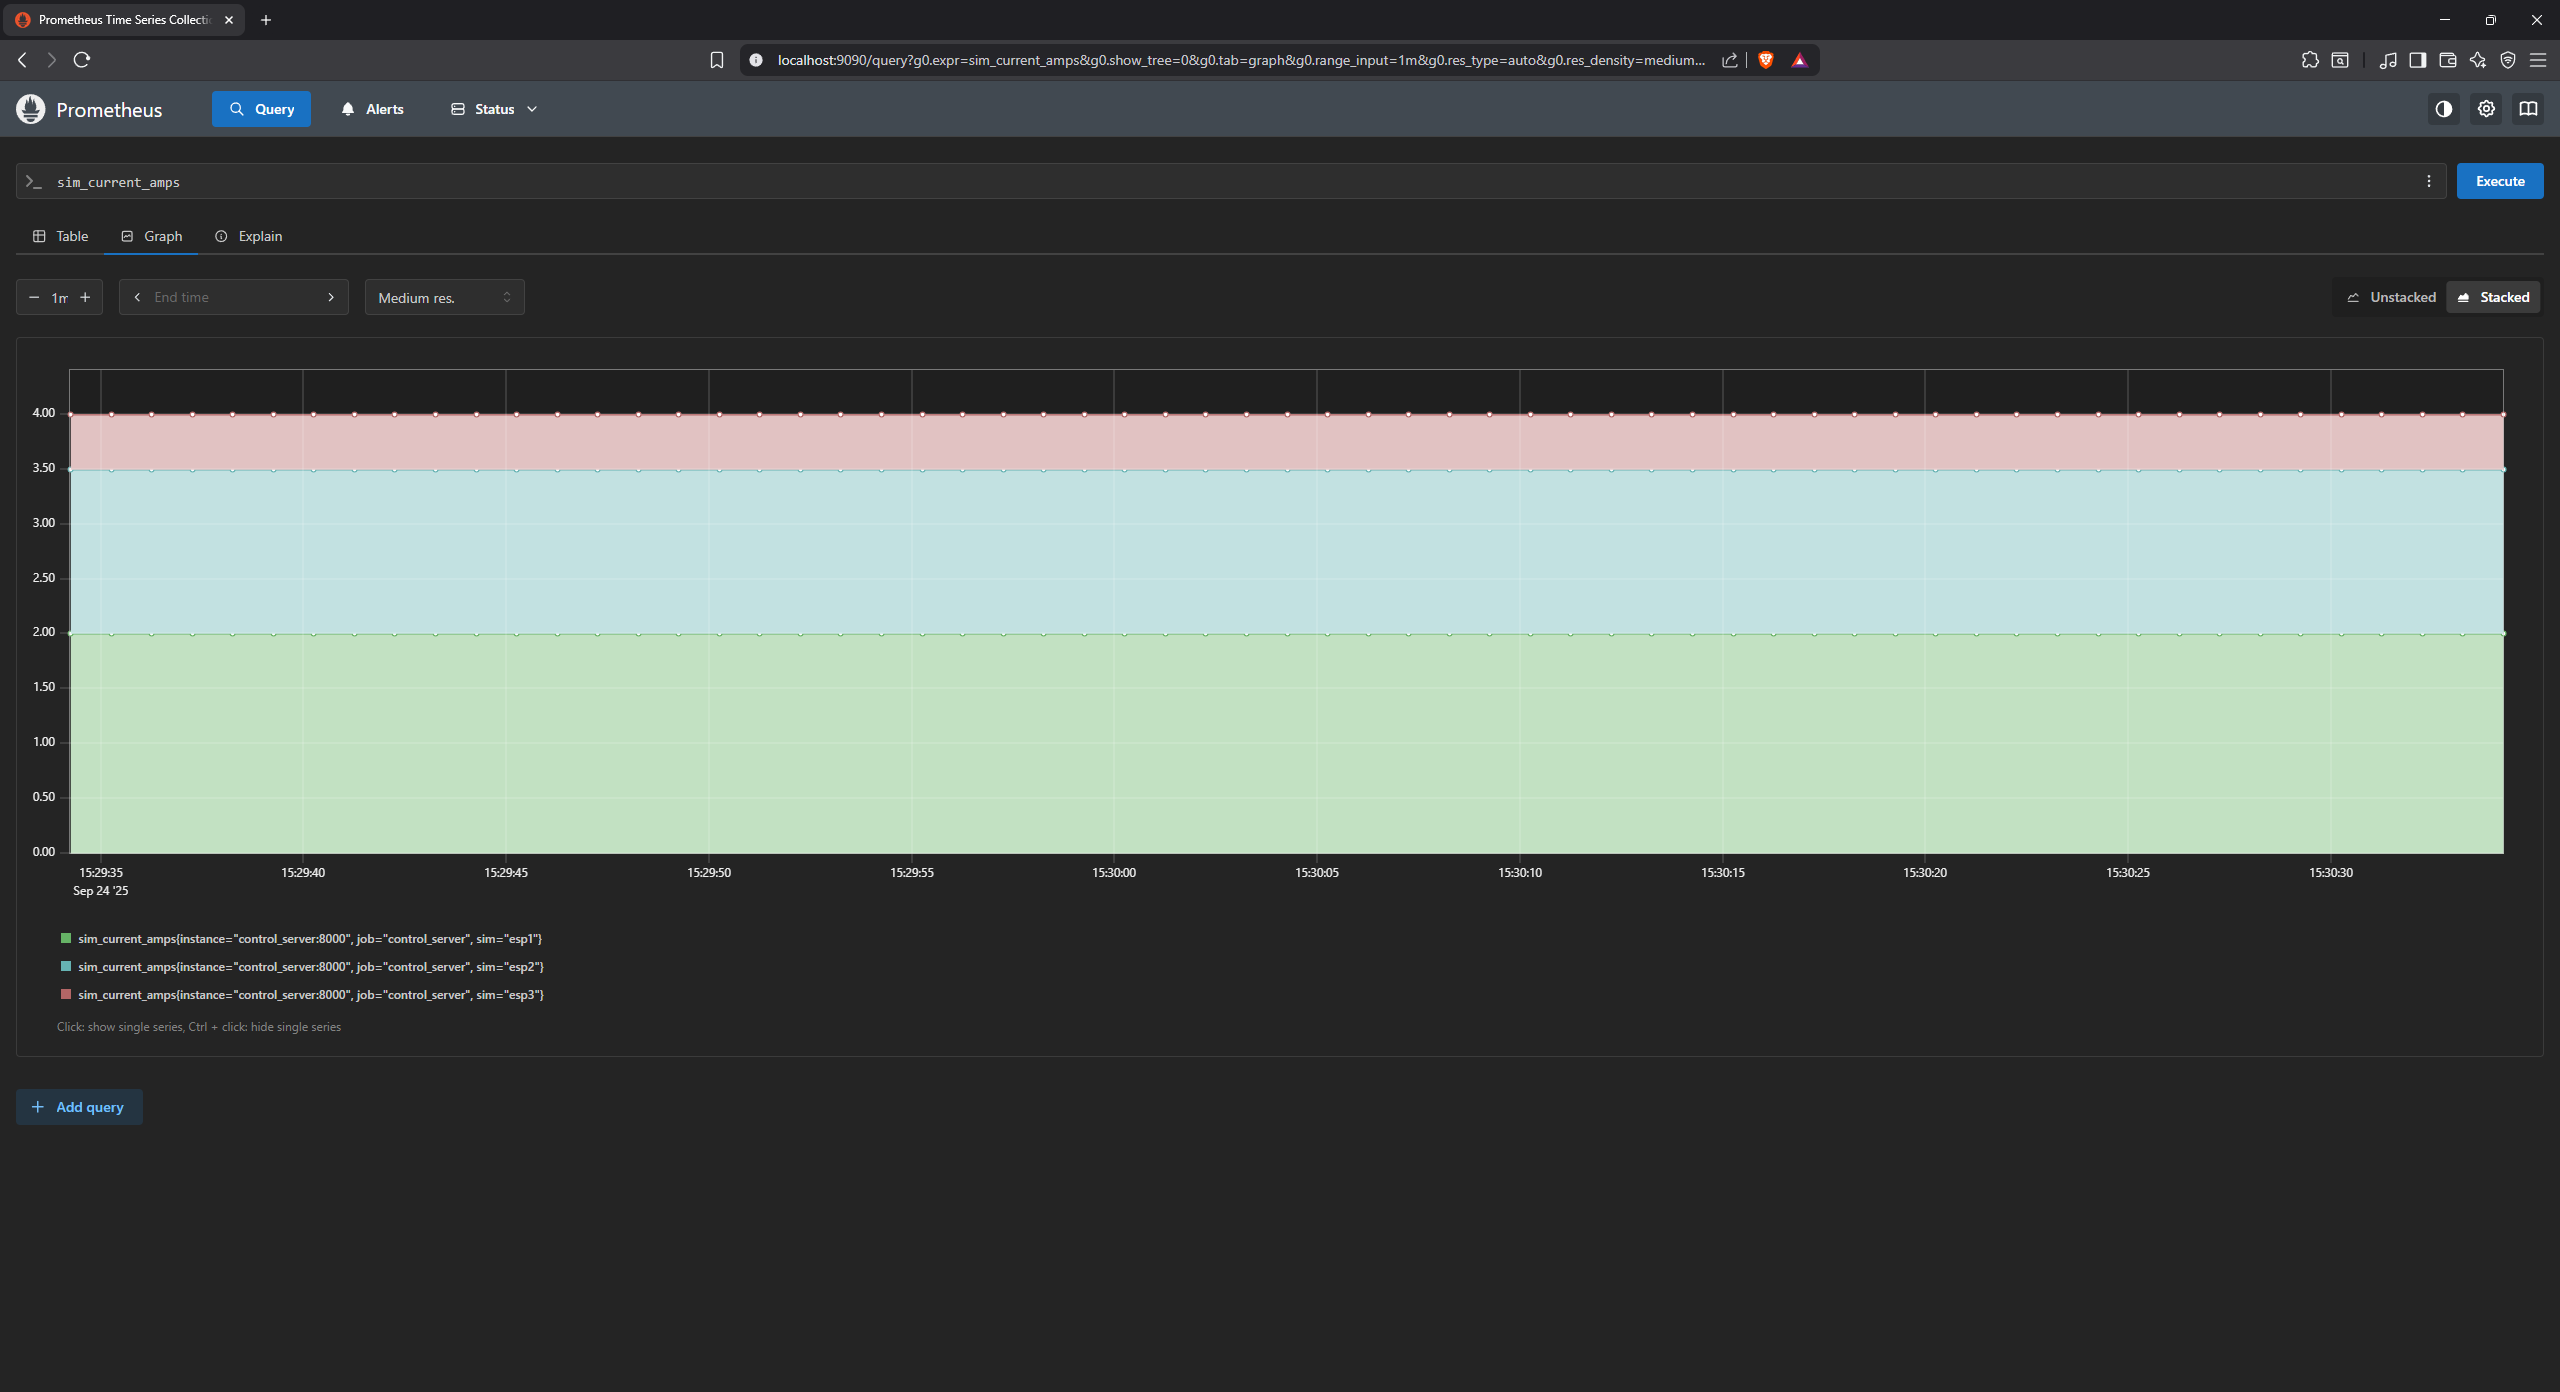
\includegraphics[width=1\textwidth]{figures/undercap_2.png}
    \caption{Alulterhelt eset}
    \label{fig:undercap}
\end{figure}

\subsection{Túlterhelés, azonos igények: fair 3/3/3}
\textbf{Bemenetek:}\\ \texttt{ALLOC\_MAX\_TOTAL=9}, \texttt{BREAKER\_MAX\_TOTAL=12}, 
\texttt{BREAKER\_MIN\_TOTAL=2}; ESP1=50 A, ESP2=50 A, ESP3=50 A.\\
\textbf{Lépések:}\\ START, várakozás \(\sim\) 2--3 ciklus.\\
\textbf{Várt eredmény:}\\ \(\lambda=9/3=3\) A \(\Rightarrow\) \(\mathrm{effective}=[3,3,3]\), Sum \(=9\) A.\\
\textbf{Siker:}\\ grafikonon három azonos szint \(\approx 3\) A; \texttt{/status} 
és \texttt{output.txt} szerint \texttt{cap}\(=3\) A mindháromnál.

\begin{figure}[H]
    \centering
    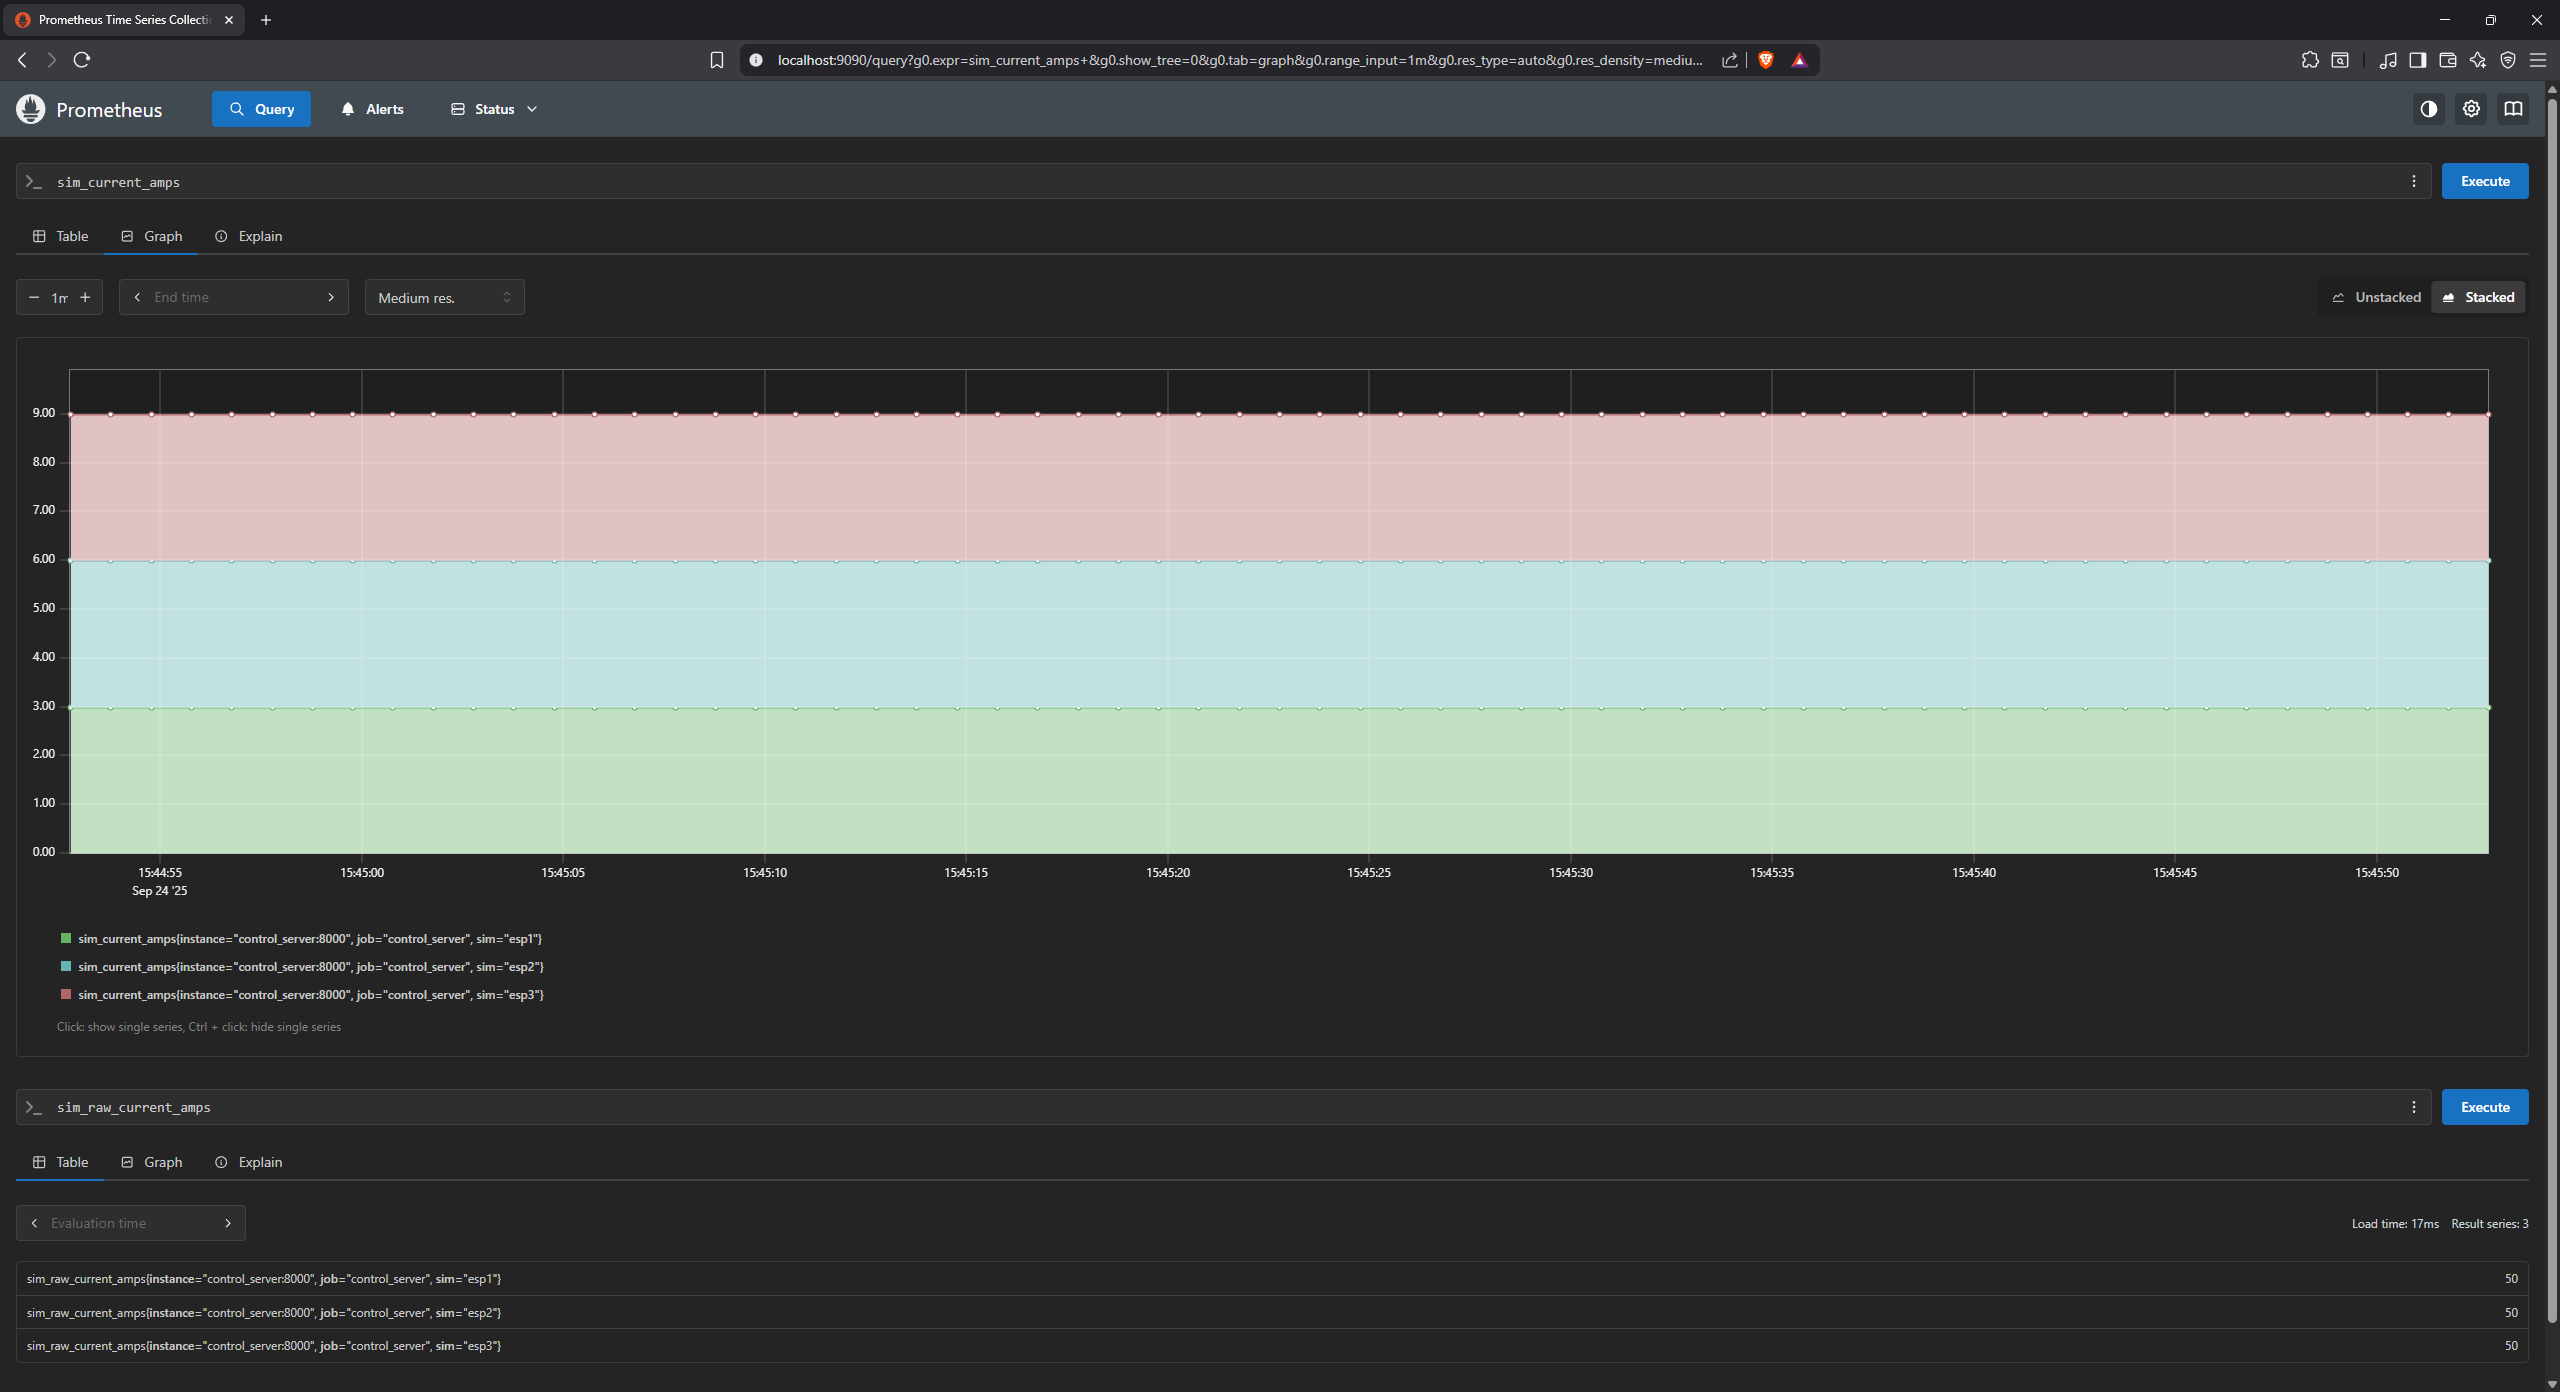
\includegraphics[width=1\textwidth]{figures/túlterhelés_3.png}
    \caption{Túlterhelt eset}
    \label{fig:Túlterhelt}
\end{figure}

\subsection{Dinamikus újraelosztás: a nagy felhasználó kap teret}
\textbf{Bemenetek:}\\ \texttt{ALLOC\_MAX\_TOTAL=90}, \texttt{BREAKER\_MAX\_TOTAL=120}, 
\texttt{BREAKER\_MIN\_TOTAL=10}. Menetrendek: \\
ESP1: \(0\) s \(\to 50\) A, \(60\) s \(\to 10\) A; \;
ESP2: \(0\) s \(\to 50\) A, \(60\) s \(\to 10\) A; \;
ESP3: \(0\) s \(\to 50\) A, \(60\) s \(\to 100\) A.\\
\textbf{Lépések:}\\ Reset \(t{=}0\), START, megfigyelés \(0..80\) s.\\
\textbf{Várt eredmény:}\\ \(0..60\) s: \([30,30,30]\), Sum \(=90\) A; \(60+\) s: \([10,10,70]\), Sum \(=90\) A.\\
\textbf{Siker:}\\ a grafikon két helyre áll be: előbb \(30\)/\(30\)/\(30\), majd \(10\)/\(10\)/\(70\).

\begin{figure}[H]
    \centering
    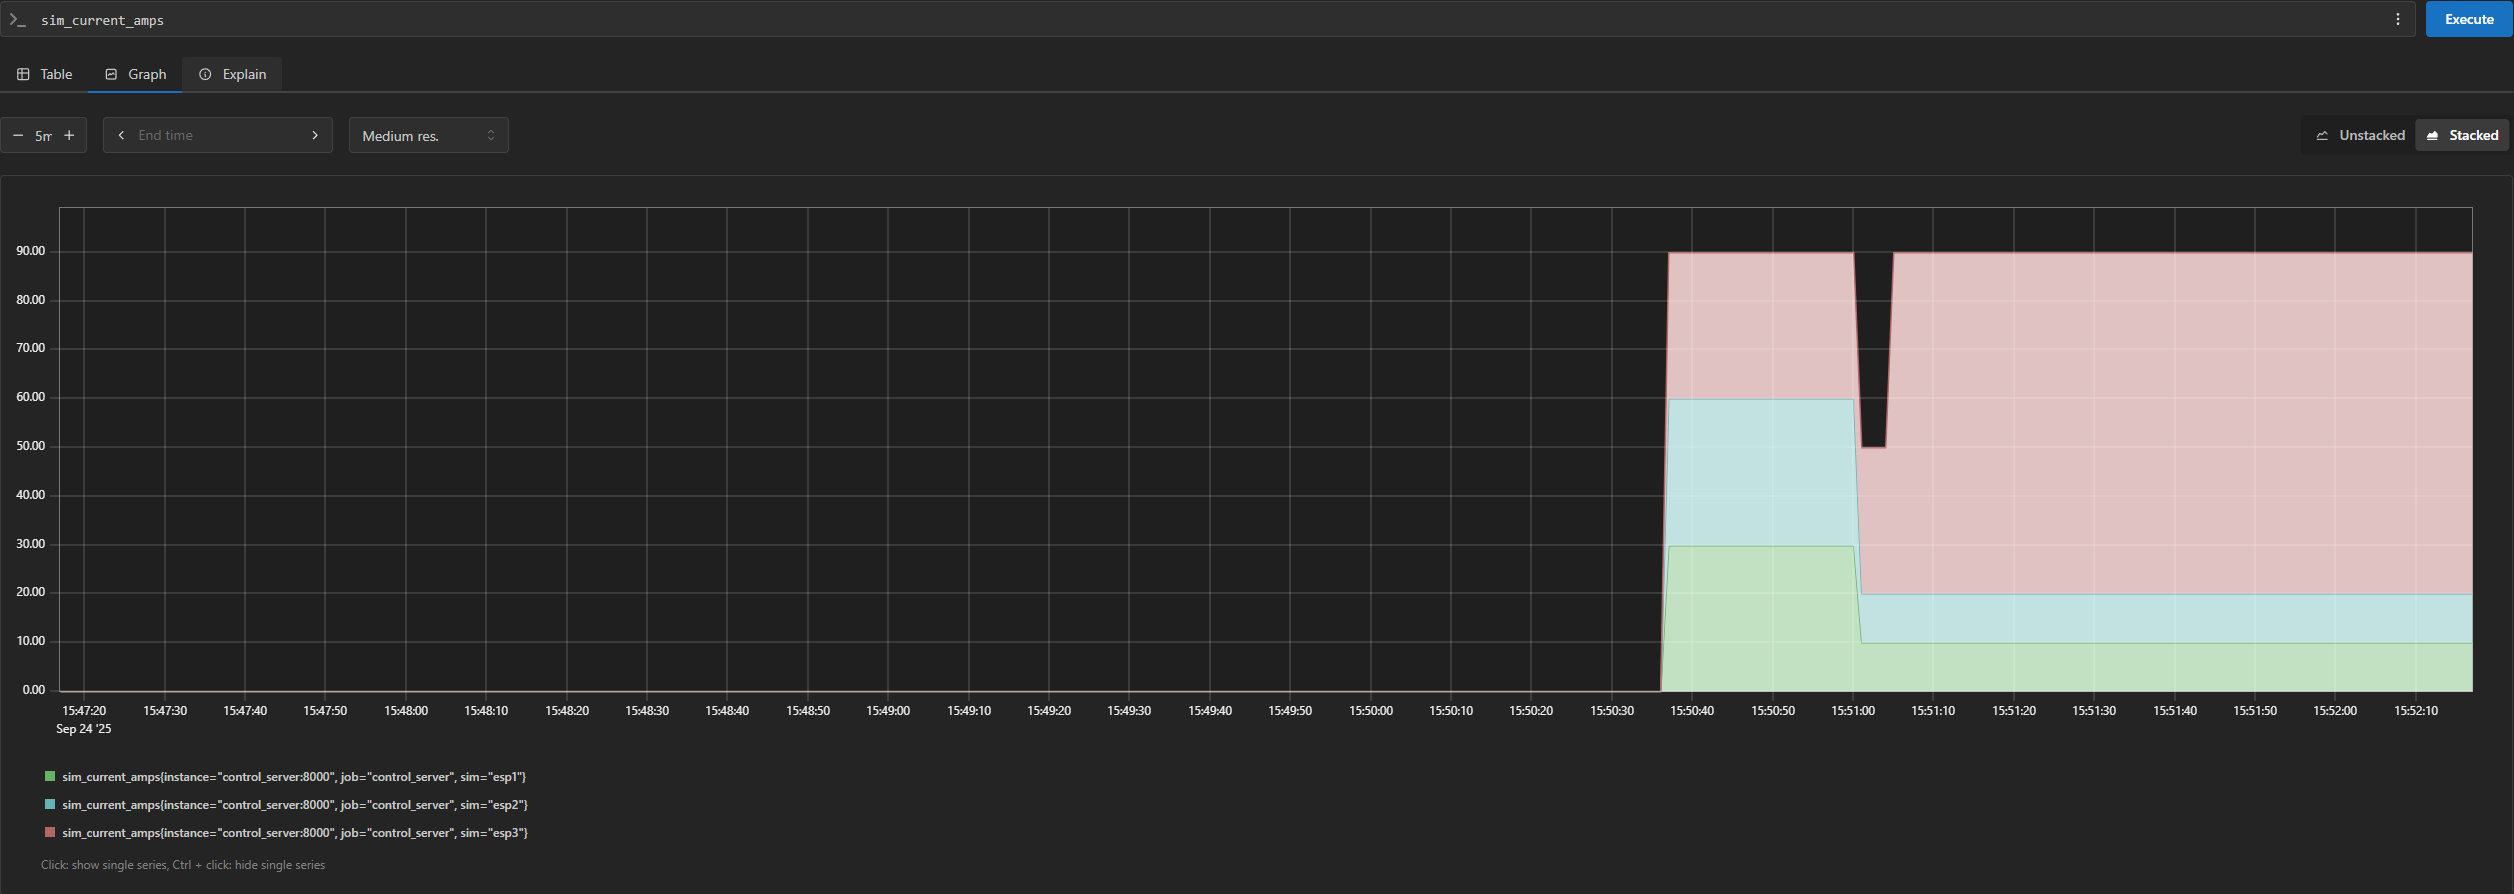
\includegraphics[width=1\textwidth]{figures/dinamikus újraelosztás_4_1.png}
    \caption{Dinamikus újraelosztás áramerősség}
    \label{fig:dynamic_reallocation_1}
\end{figure}

\begin{figure}[H]
    \centering
    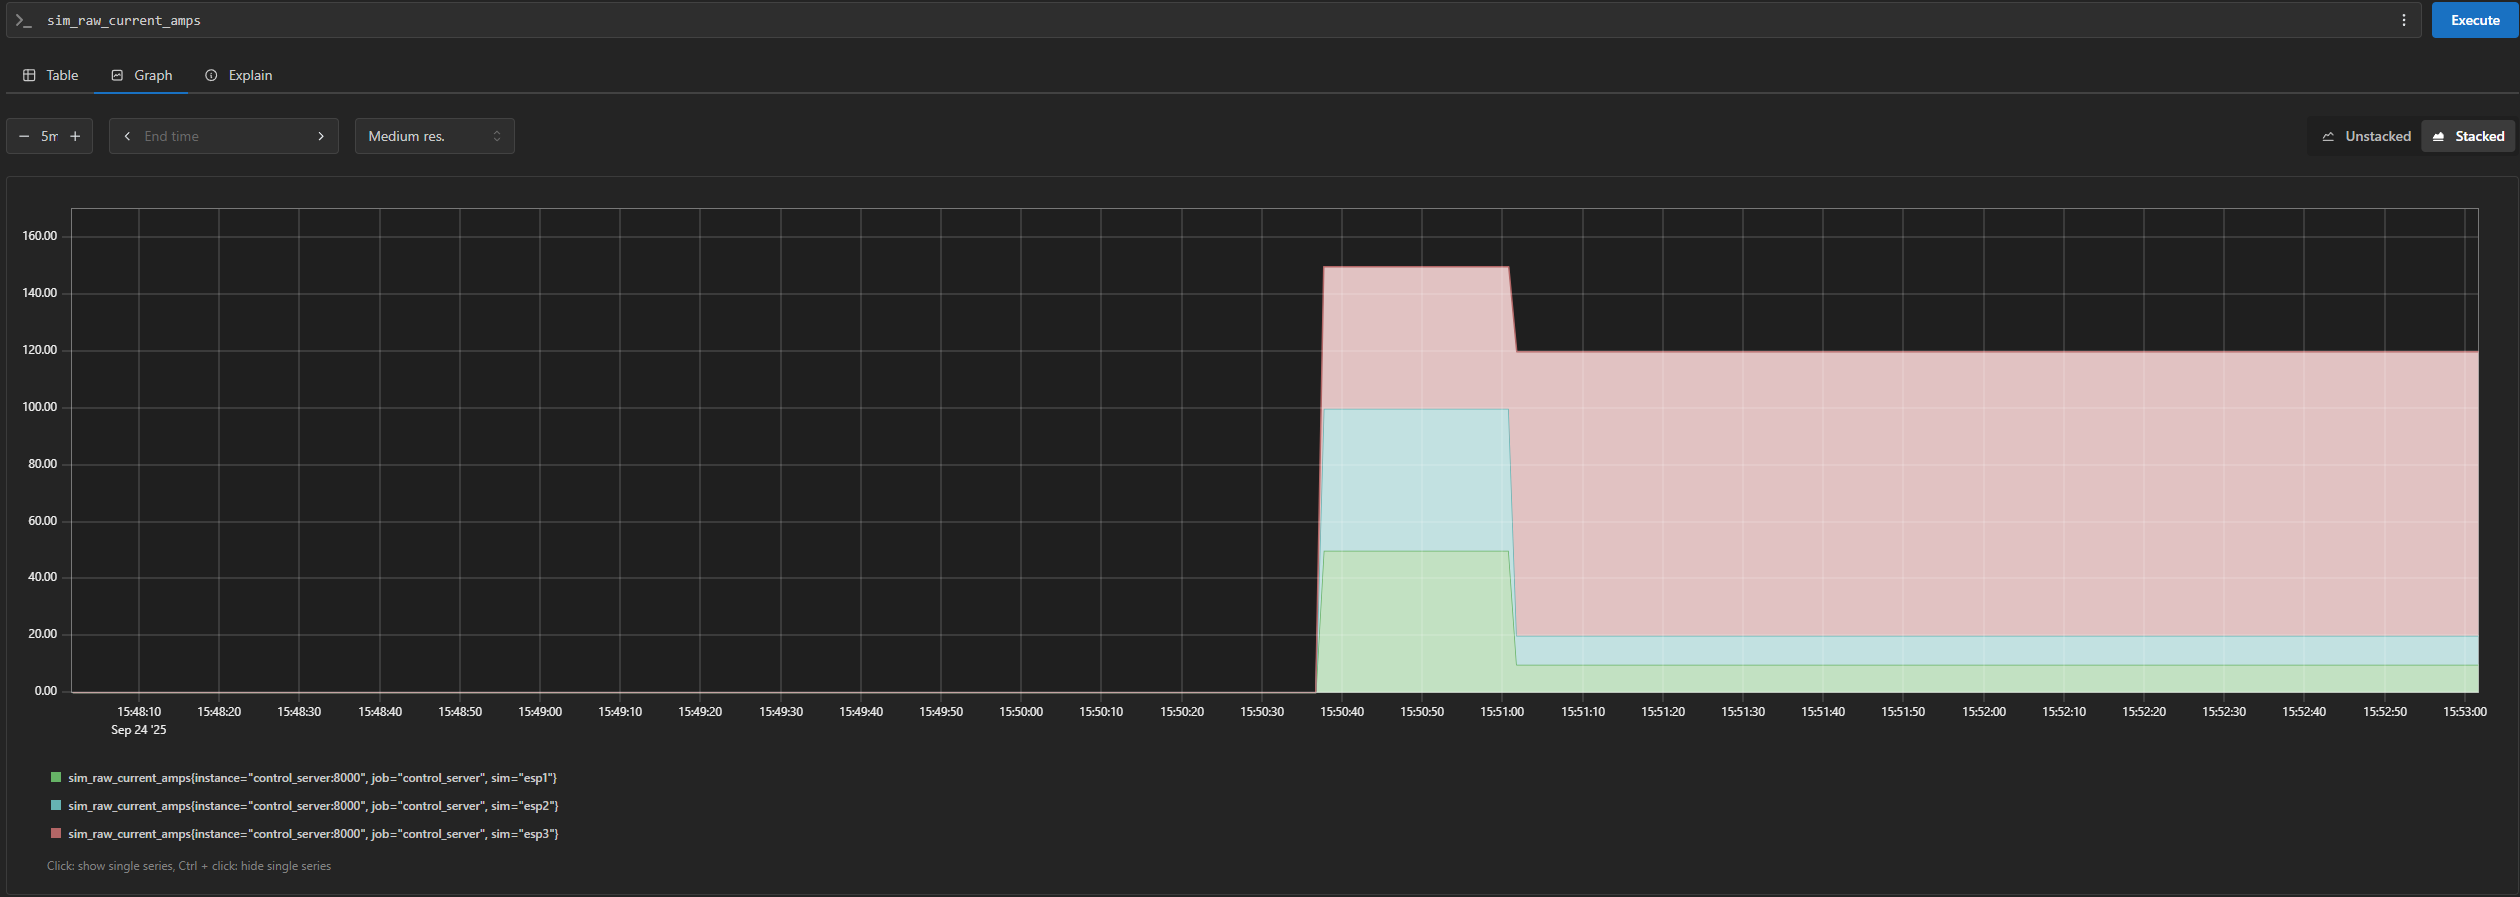
\includegraphics[width=1\textwidth]{figures/dinamikus újraelosztás_4_2.png}
    \caption{Dinamikus újraelosztás igények}
    \label{fig:dynamic_reallocation_2}
\end{figure}

\subsection{Megszakító hiszterézis}
\textbf{Bemenetek:}\\ \texttt{ALLOC\_MAX\_TOTAL=50}, \texttt{BREAKER\_MAX\_TOTAL=6}, 
\texttt{BREAKER\_MIN\_TOTAL=3}. Menetrendek: \\
ESP1: \(0\) s \(\to 2.0\) A, \(40\) s \(\to 0.5\) A; \;
ESP2: \(0\) s \(\to 5.0\) A, \(40\) s \(\to 0.5\) A; \;
ESP3: \(0\) s \(\to 0.0\) A.\\
\textbf{Lépések:}\\ Reset \(t{=}0\), START, megfigyelés \(0..60\) s.\\
\textbf{Várt eredmény:}\\ \(0..40\) s Sum \(=7\) A \(\Rightarrow\) \texttt{off}; \(40+\) 
s Sum \(=1\) A \(\Rightarrow\) \texttt{on}.\\
\textbf{Siker:}\\ \texttt{breakers= 0 s:off, 40 s:off} \(\to\) \texttt{on,\ on} váltás 
az \texttt{output.txt}-ben és \texttt{/status}-ban.

\begin{figure}[H]
    \centering
    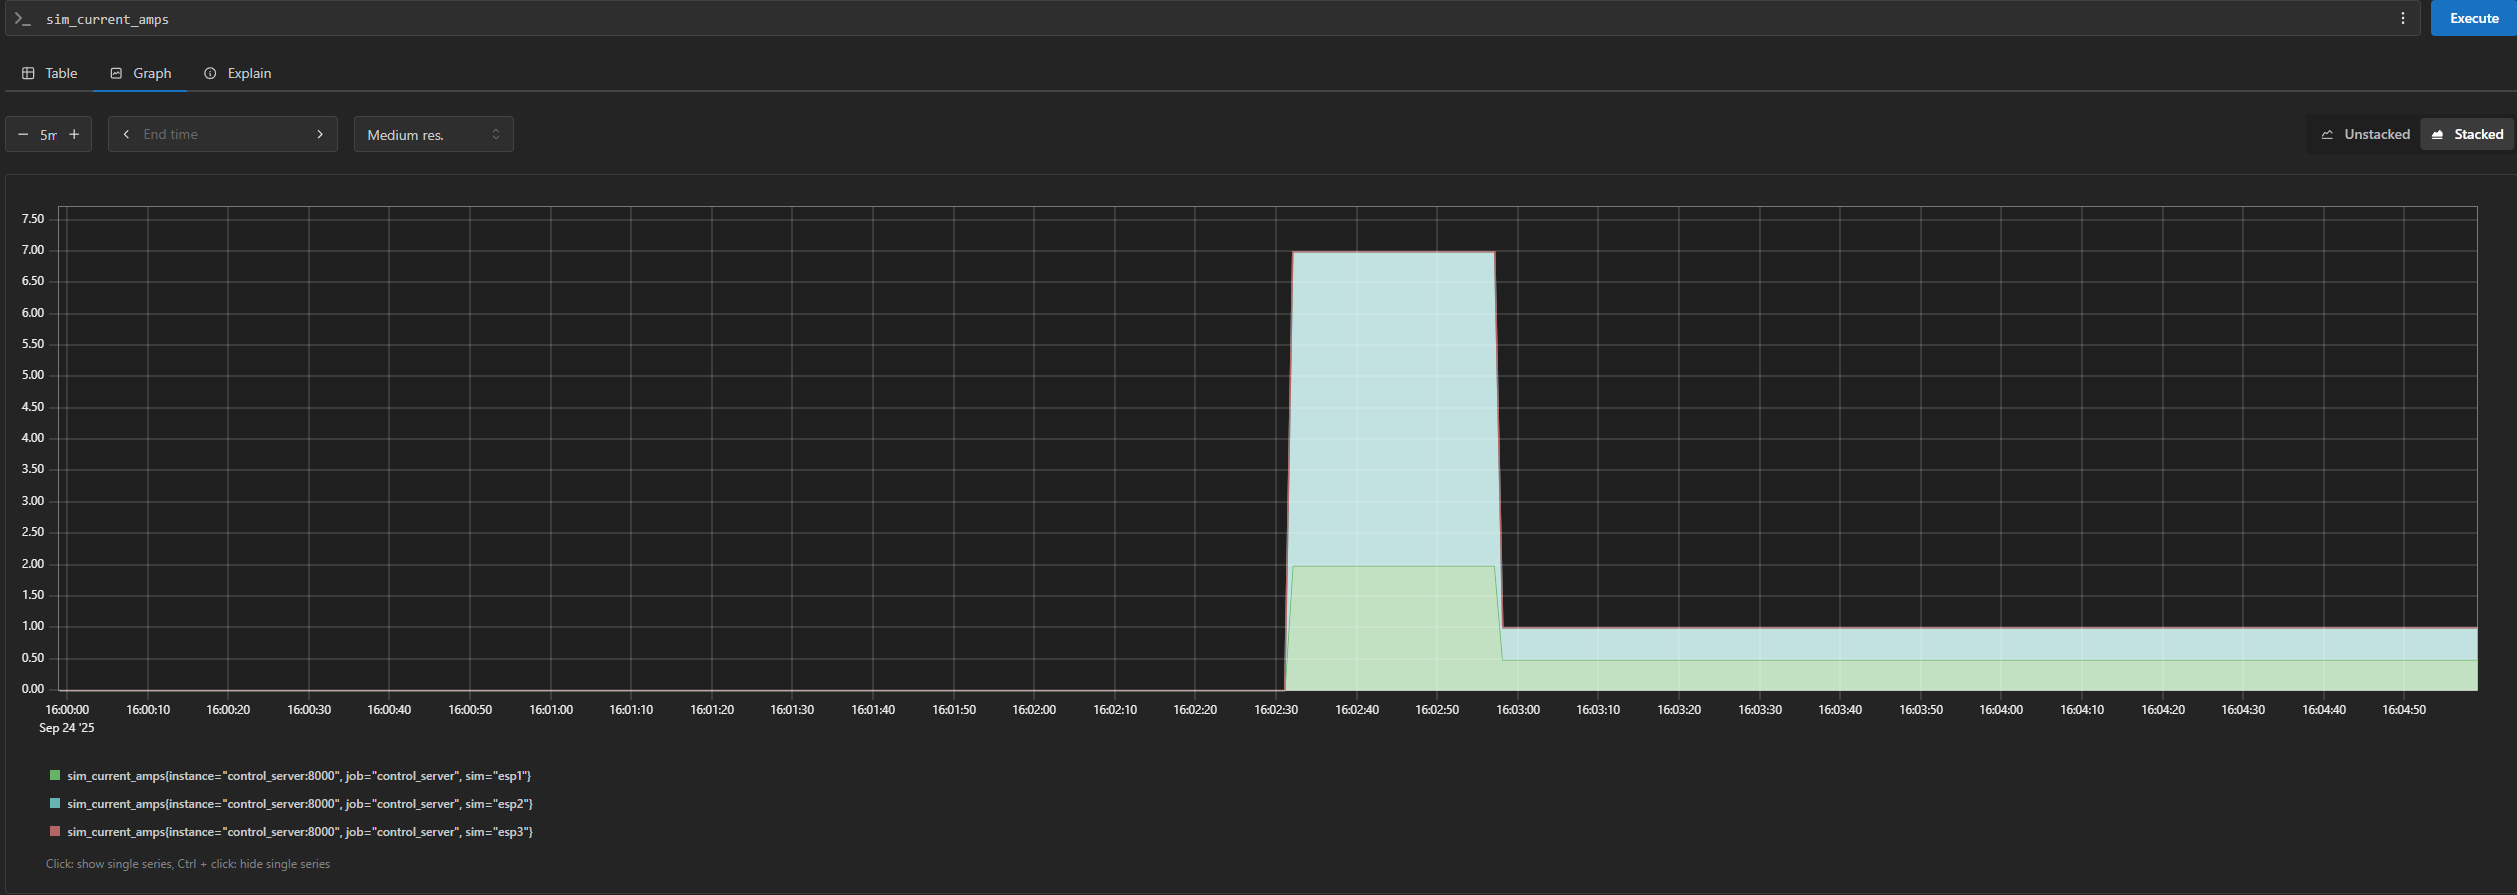
\includegraphics[width=1\textwidth]{figures/megszakító_5_1.png}
    \caption{Megszakító áramerősség}
    \label{fig:megszakító_1}
\end{figure}

\begin{figure}[H]
    \centering
    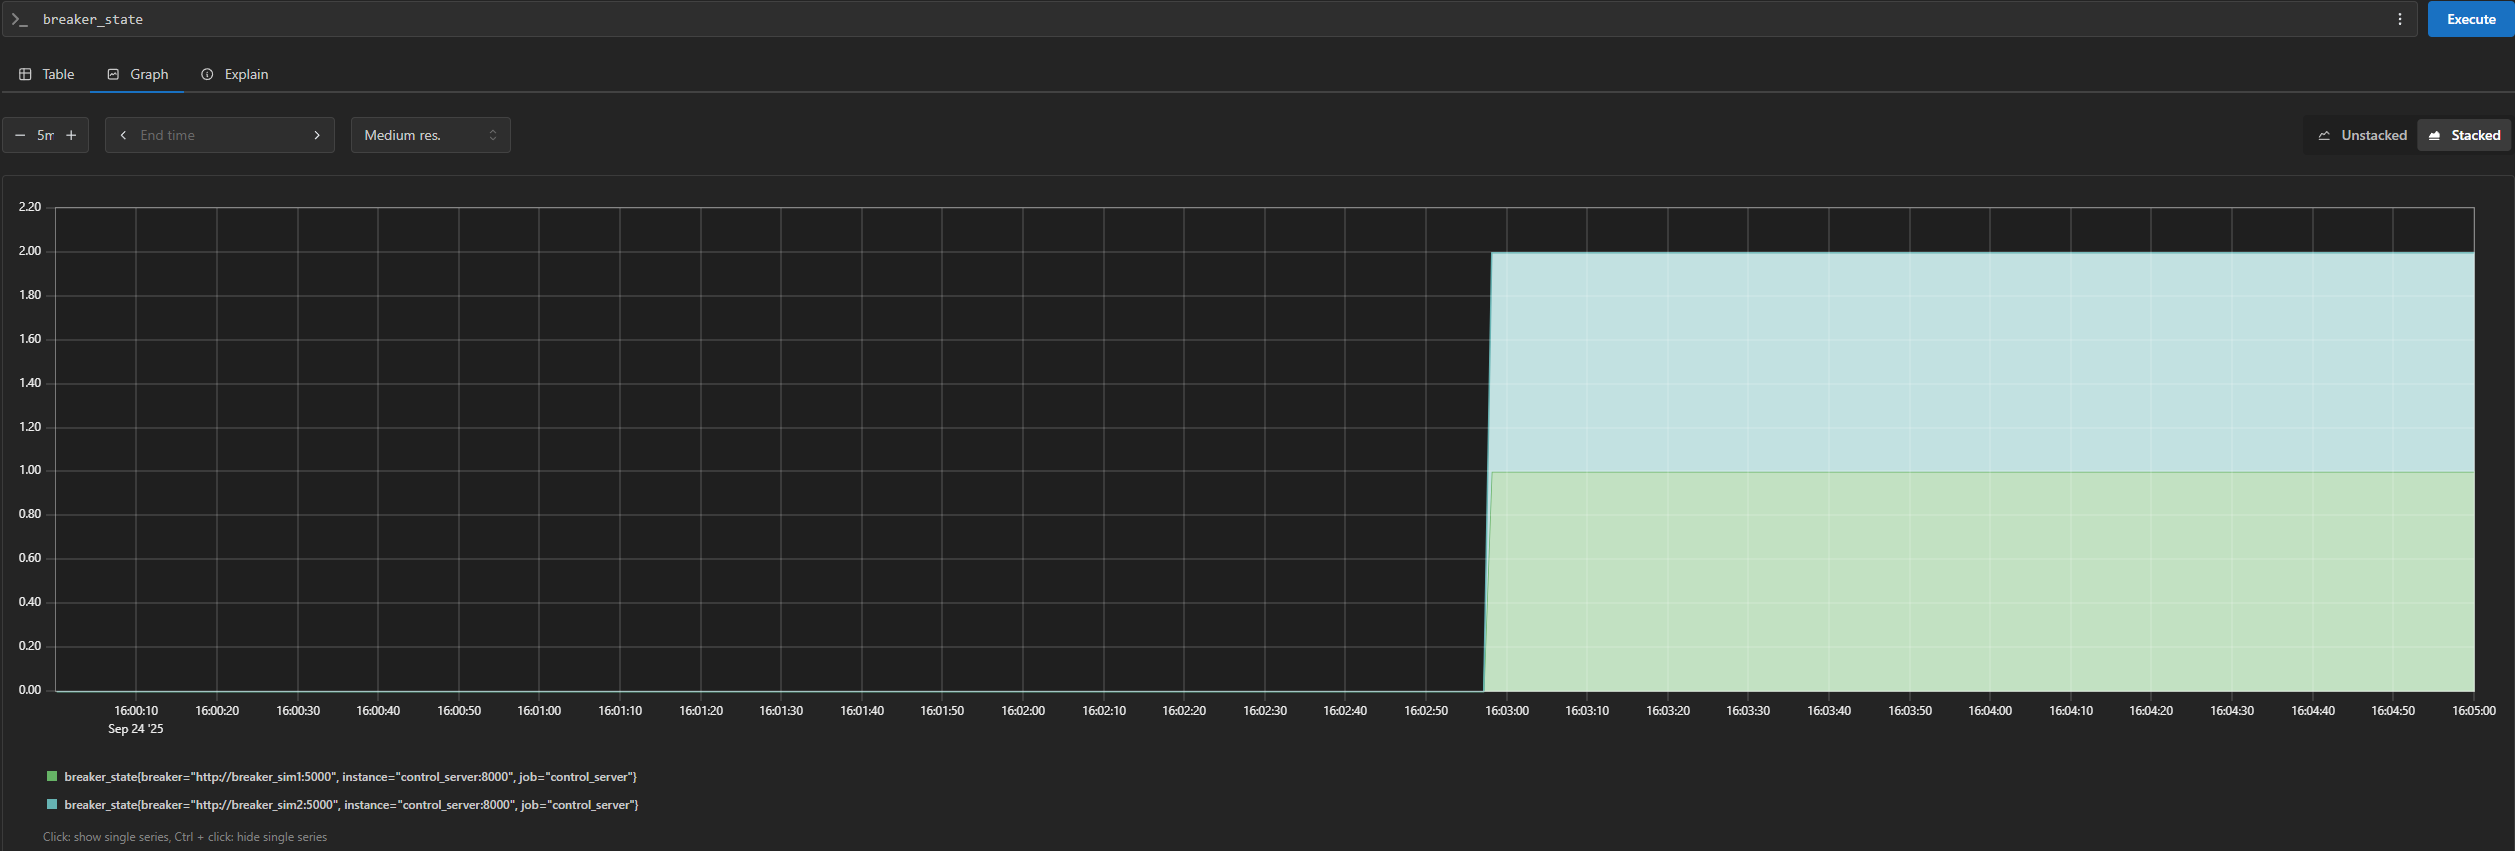
\includegraphics[width=1\textwidth]{figures/megszakító_5_2.png}
    \caption{Megszakító állapotok}
    \label{fig:megszakító_2}
\end{figure}

\subsection{STOPPED invariánsok}
\textbf{Bemenetek:}\\ induljunk a 3.\ szcenárió állapotából (3/3/3 cap).\\
\textbf{Lépések:}\\ \texttt{STOPPED} módba váltás; módosítsuk \texttt{ALLOC\_MAX\_TOTAL=6}-ra, 
ESP1 menetrendjét \(1\) A-ra; várjunk \(\sim\) 2 ciklust.\\
\textbf{Várt eredmény:}\\ a cap-ek és a megszakítóállapot \textbf{nem} változik (\texttt{STOPPED} 
alatt nem történik beavatkozás).\\
\textbf{Siker:}\\ \texttt{/status.sim\_state=STOPPED}; a \texttt{cap} és a \texttt{breakers} mezők változatlanok.

\begin{figure}[H]
    \centering
    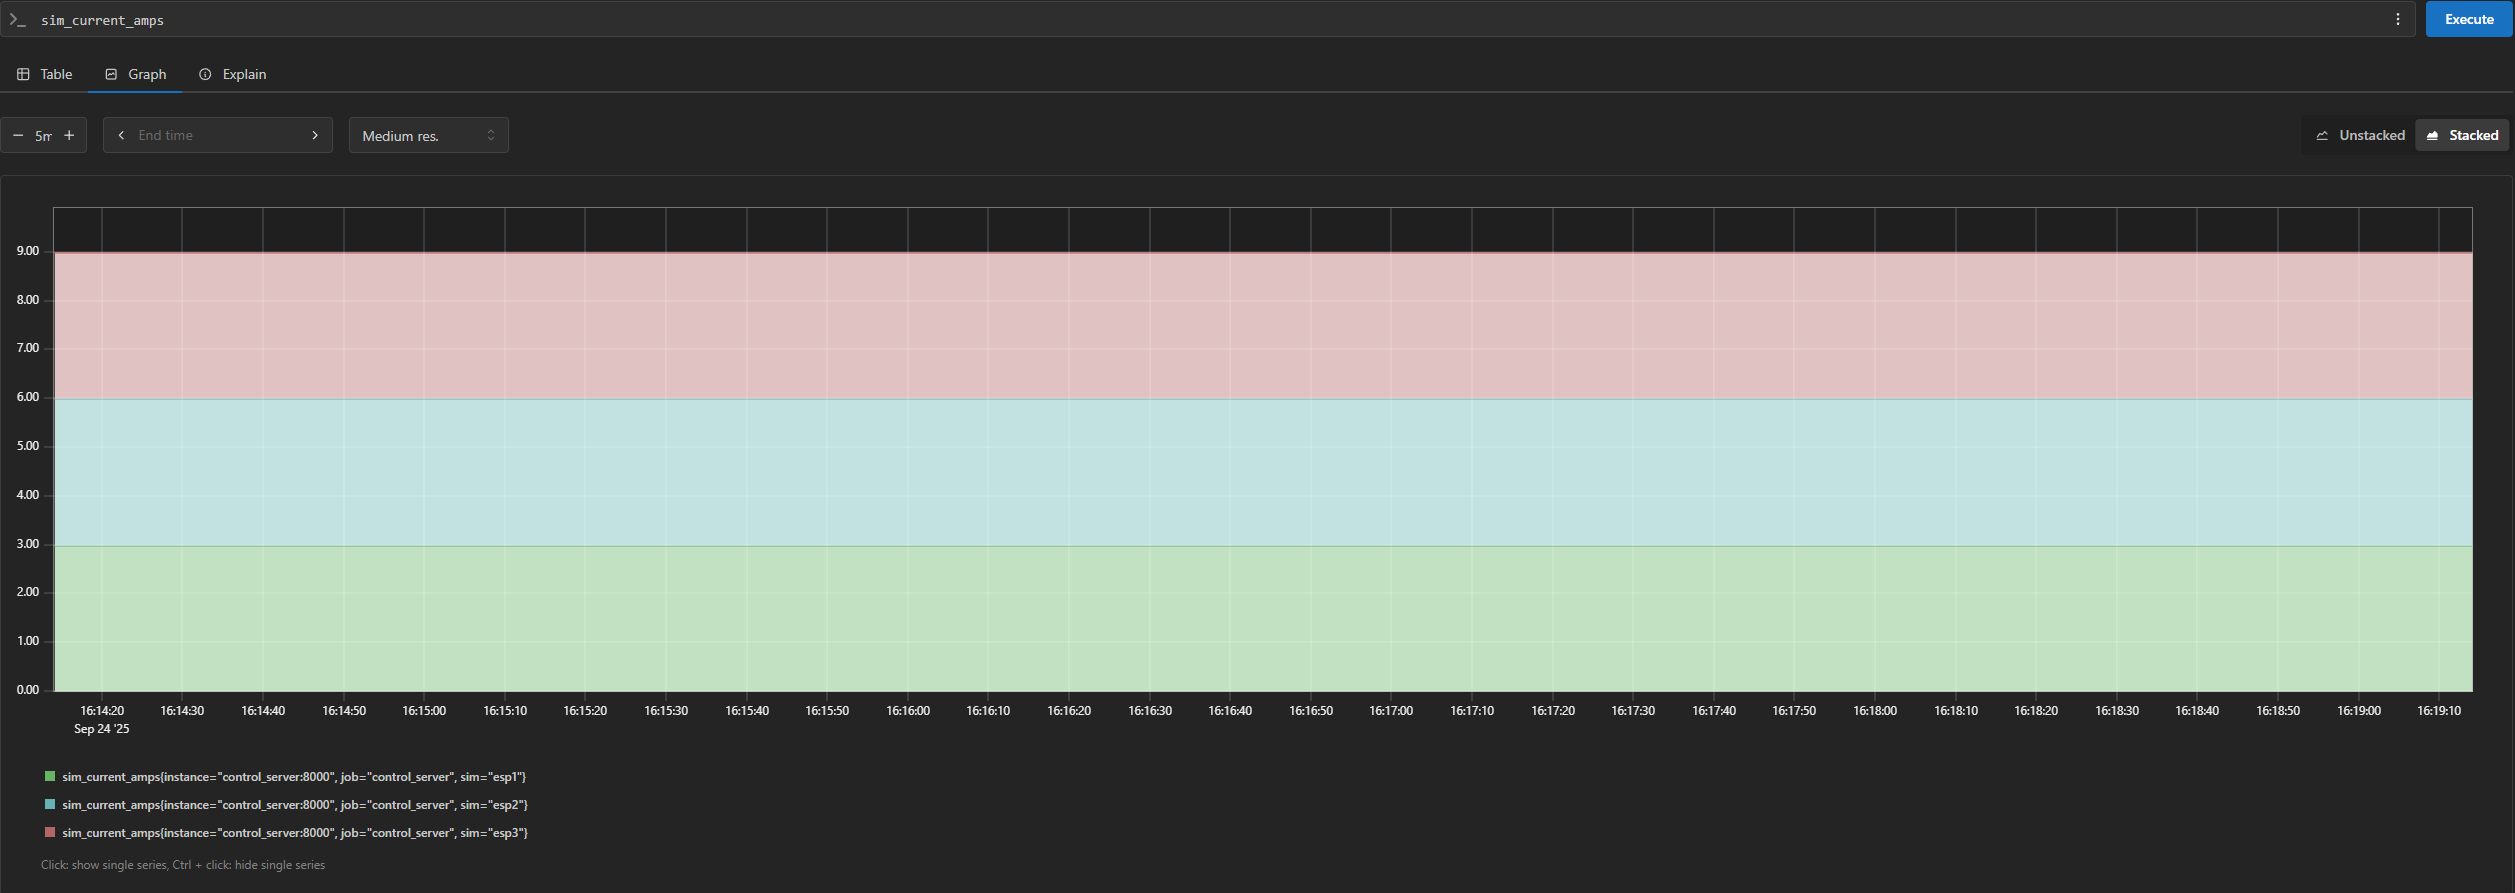
\includegraphics[width=1\textwidth]{figures/stop_6_1.png}
    \caption{stopped állapot áramerősség}
    \label{fig:stop_1}
\end{figure}

\begin{figure}[H]
    \centering
    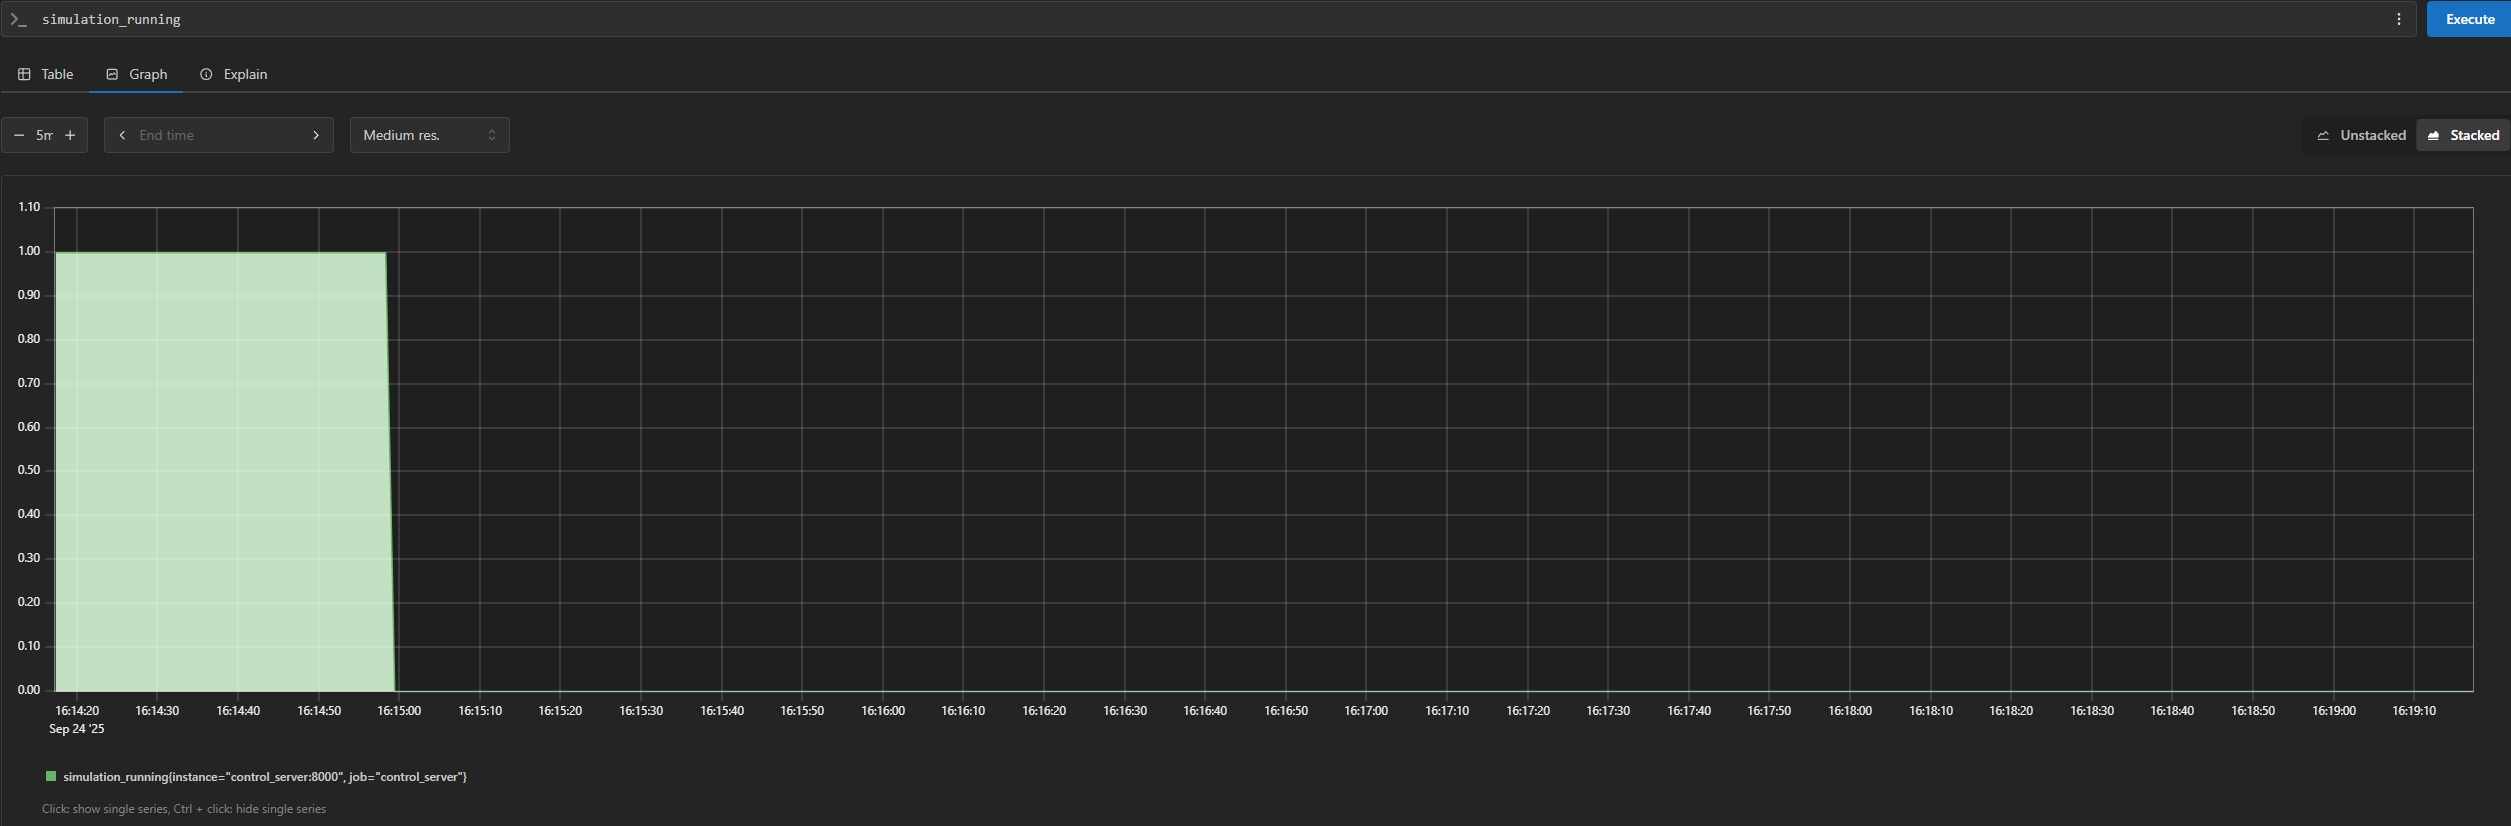
\includegraphics[width=1\textwidth]{figures/stop_6_2.png}
    \caption{stopped állapot állapotok}
    \label{fig:stop_2}
\end{figure}

\begin{figure}[H]
    \centering
    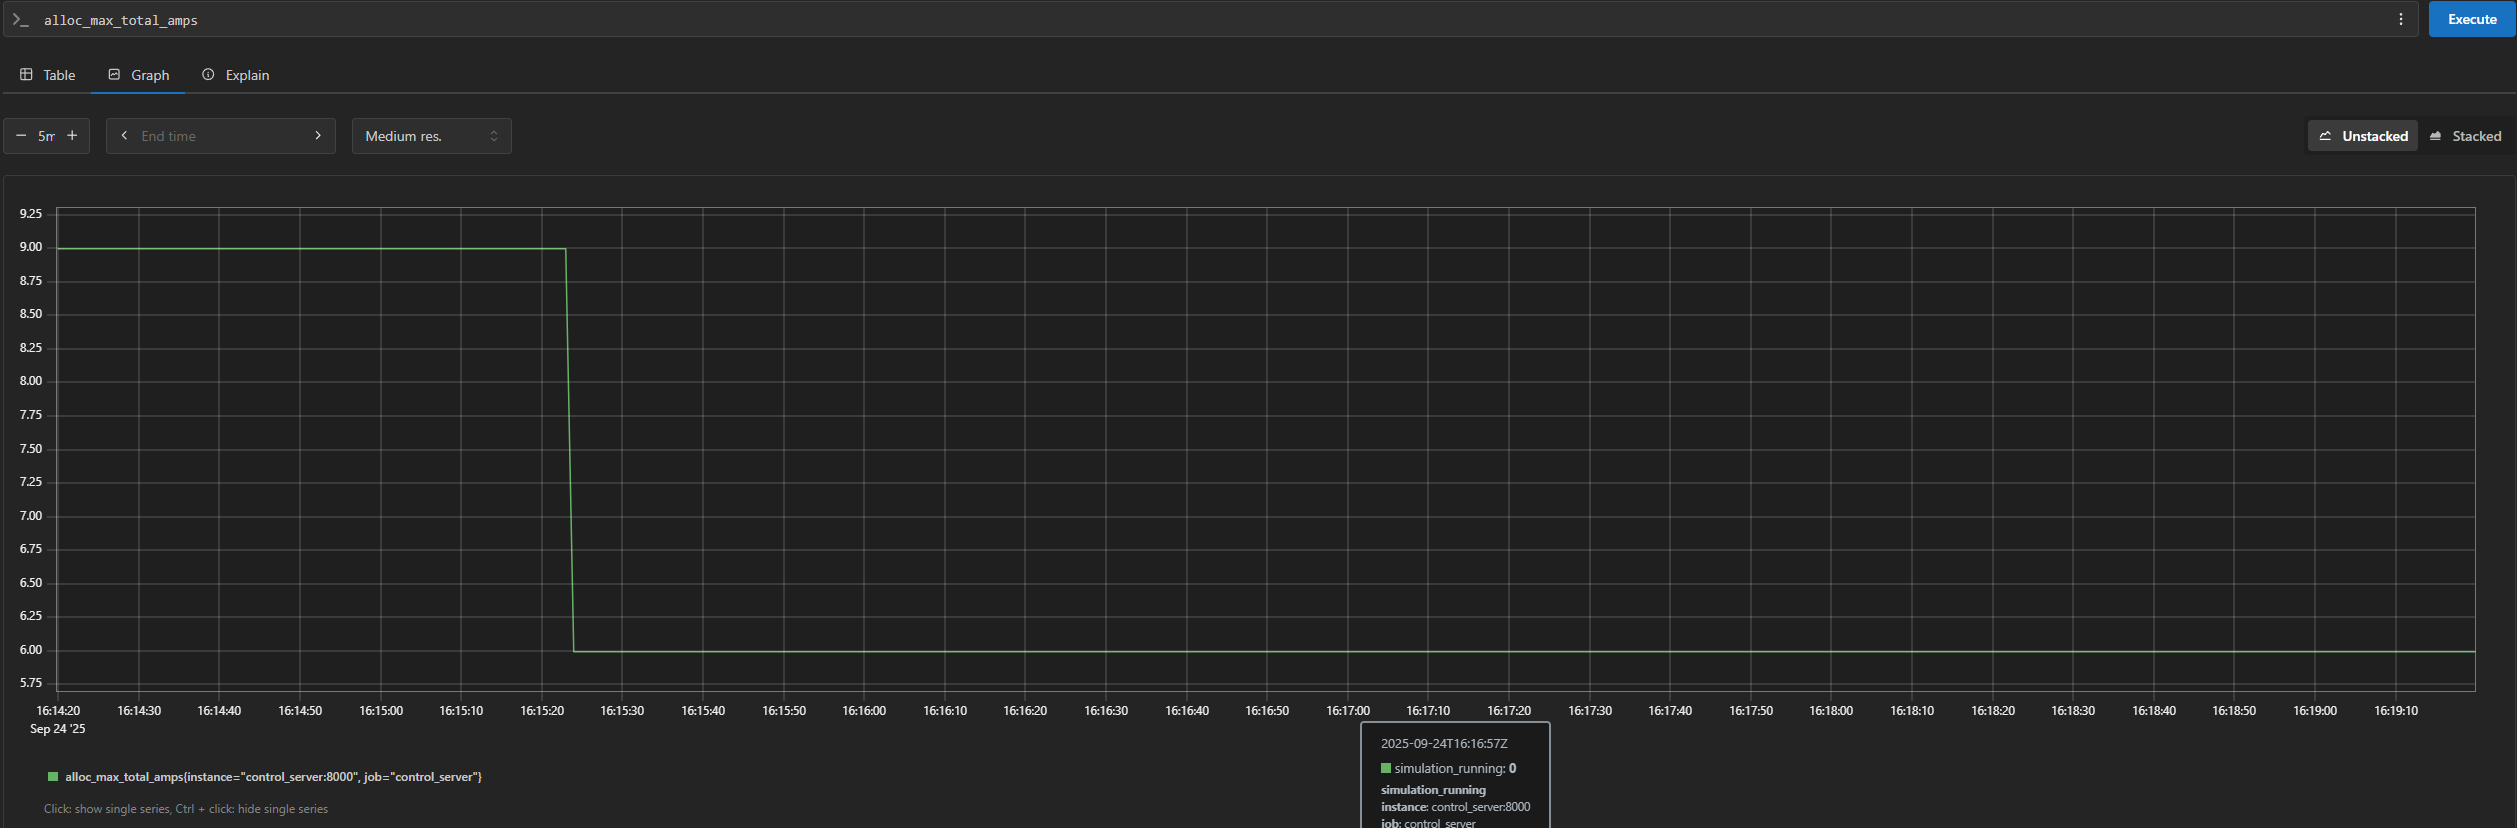
\includegraphics[width=1\textwidth]{figures/stop_6_3.png}
    \caption{stopped állapot maximális áramok}
    \label{fig:stop_3}
\end{figure}

\section*{Összegzés}
A tesztek ellenőrzik, hogy (i) az allokáció a max-min fair elvet követi-e, (ii) 
a megszakító hiszterézise a küszöbértékekhez képest működik-e, (iii) a \texttt{STOPPED}
állapot működik-e, és (iv) a rendszer minden ciklusban önmagát leíró idősoros naplót állít elő.
Ezek együttesen biztosítják az elvárt funkcio nális helyességet és transzparens viselkedést.
